\usetikzlibrary{calc}
\usetikzlibrary{math} % for \tikzmath
\usetikzlibrary{decorations.pathmorphing} % for snake, coil, zigzag
\tikzset{>=latex} % set default arrow head as latex

% COLORS
\colorlet{leptoncol}{green!70!black}
\colorlet{quarkcol}{blue!85!cyan!80!black}
\colorlet{photoncol}{yellow!80!orange!90!black}
\colorlet{exocol}{red!80!black}
\colorlet{anycol}{blue!80!cyan!60!red!95!black!90}

% STYLES
\tikzstyle{label}=[align=center,rounded corners=3pt] %fill=blue!60!cyan!80!black!15,
\tikzstyle{legend}=[draw=black,thick,rounded corners=3pt] %,fill=blue!60!cyan!80!black!15
\tikzstyle{entry}=[right=1pt,inner sep=4pt]
\tikzstyle{particle}=[anycol,very thick,line cap=round]
\tikzstyle{lepton}=[particle,leptoncol]
\tikzstyle{quark}=[particle,quarkcol]
\tikzstyle{track}=[quark,thick]
\tikzstyle{photon}=[particle,photoncol,decorate,decoration={
  snake,amplitude=.4mm,segment length=2.5mm,post length=1mm}]
\tikzstyle{charged exo}=[particle,exocol]
\tikzstyle{neutral exo}=[charged exo,dashed]

% JET CONE
\newcommand\jetcone[6][quarkcol]{{
  \pgfmathanglebetweenpoints
    {\pgfpointanchor{#2}{center}}
    {\pgfpointanchor{#3}{center}}%
  \pgfmathsetmacro\oang{#4/2}       % half‑opening angle
  \edef\e{#5}                       % eccentricity
  \def\tmpL{tmpL-#2-#3}             % unique coordinate name
  \edef\vang{\pgfmathresult}        % direction of axis
  \tikzmath{%
    coordinate \jetvec;             % ← was \C
    \jetvec = (#2)-(#3);            % vector OV
    \x    = veclen(\jetvecx,\jetvecy)*\e*sin(\oang)^2;
    \y    = tan(\oang)*(veclen(\jetvecx,\jetvecy)-\x);
    \a    = veclen(\jetvecx,\jetvecy)*sqrt(\e)*sin(\oang);
    \b    = veclen(\jetvecx,\jetvecy)*tan(\oang)*sqrt(1-\e*sin(\oang)^2);
    \angb = acos(sqrt(\e)*sin(\oang));
  }
  \coordinate (#2-v) at ($(#2)+(\vang:1pt)$); 
  \coordinate (\tmpL) at 
    ($(#3)-(\vang:\x pt)+(\vang+90:\y pt)$); 
  \draw[thin,#1!50!black,fill=#1!80!black!50,line cap=round,rotate=\vang]
    (#2) -- (\tmpL) arc(180-\angb:180+\angb:{\a pt} and {\b pt}) -- (#2);
  \draw[thin,#1!50!black,rotate=\vang,
        top color=#1!60!black!60,bottom color=#1!50!black!75,
        shading angle=\vang]
    (#3) ellipse({\a pt} and {\b pt});
  #6 % extra tracks
  \draw[thin,#1!50!black,rotate=\vang,fill opacity=0.80,
        top color=#1!90!black!20,bottom color=#1!50!black!50,
        line cap=round,shading angle=\vang]
    (#2) -- (\tmpL) arc(180-\angb:180+\angb:{\a pt} and {\b pt}) -- (#2);
}}

% DETECTOR
\def\scale{1.6} % scale diagrams
\def\keepseg#1#2{% % return boolean if detector segment falls outside mask
  (\mask==0 || (#2>\angmin-4 && #1<\angmax+4) || (#2>\angmin+356 && #1<\angmax+364))
}
\tikzset{
  pics/detector/.style args={#1:#2}{
    code={
  
  % MASK except segment
  \pgfmathsetmacro\mask{#1!=#2}
  \pgfmathsetmacro\angmin{#1>=0 ? #1 : 360+#1}
  \pgfmathsetmacro\angmax{#2>=0 ? #2 : 360+#2}
  \message{^^JDetector: 1=#1, 2=#2, angmin=\angmin, angmax=\angmax, mask=\mask}
  \begin{scope}[pic actions]
  
  % CLIP
  \ifnum\mask=1 % clip detector segment
    %\draw[thick,black] (0,0) -- (#1:2.3) arc(#1:#2:2.3) -- cycle;
    %\clip (0,0) -- (\angmin:2.3) arc(\angmin:\angmax:2.3) -- cycle;
    \clip (0,0) -- (#1:2.3) arc(#1:#2:2.3) -- cycle;
  \fi
  
  % PIXEL TRACKER (PBIX)
  \foreach \Rlay in {0.09,0.13,0.17,0.21}{
    \message{^^JPixel tracker: Rlay=\Rlay}
    \draw[line width=0.1] (0,0) circle(\Rlay);
  }
  
  % SILICON INNER TRACKER (TIB)
  \def\h{0.12}
  \def\w{0.010}
  \def\d{0.028}
  \foreach \Rlay/\Nlay in {0.40/30,0.55/38,0.70/46,0.85/52}{
    \message{^^JInner tracker: Rlay=\Rlay, Nlay=\Nlay}
    \foreach \i [
      evaluate={\ang=\i*(360/\Nlay);\keep=\keepseg{\ang}{\ang};}
    ] in {1,...,\Nlay}{
      \ifnum\keep=1
        \fill[rotate around={\ang+10:(\ang:\Rlay-\d)},rounded corners=0.05pt]
          (\ang:\Rlay-\d)++(-\w/2,-\h/2) rectangle++(\w,\h);
        \fill[rotate around={\ang+10:(\ang:\Rlay+\d)},rounded corners=0.05pt]
          (\ang:\Rlay+\d)++(-\w/2,-\h/2) rectangle++(\w,\h);
      \fi
    }
  }
  
  % OUTER TRACKER (TOB)
  \def\h{0.18}
  \def\w{0.011}
  \def\d{0.021}
  \foreach \Rlay/\Nlay in {1.00/21,1.12/24,1.24/27,1.36/30,1.48/33,1.64/37}{
    \message{^^JOuter tracker: Rlay=\Rlay, Nlay=\Nlay}
    \foreach \i [
      evaluate={\anga=(\i-1)*360/\Nlay;\angb=(\i-0.5)*360/\Nlay;
                \keep=\keepseg{\anga}{\angb};}
    ] in {1,...,\Nlay}{
      \ifnum\keep=1
        \fill[rotate={\anga},rounded corners=0.05pt]
          (0:\Rlay-\d-0.55*\w)++(-\w/2,-\h/2) rectangle++(\w,\h)
          (0:\Rlay-\d+0.55*\w)++(-\w/2,-\h/2) rectangle++(\w,\h);
        \fill[rotate={\angb},rounded corners=0.1pt]
          (0:\Rlay+\d-0.55*\w)++(-\w/2,-\h/2) rectangle++(\w,\h)
          (0:\Rlay+\d+0.55*\w)++(-\w/2,-\h/2) rectangle++(\w,\h);
      \fi
    }
  }
  
  % ECAL
  \def\Ntow{18}
  \def\Rin{1.85} % inner radius
  \def\Rout{2.24} % outer radius
  \message{^^JECAL: Ntow=\Ntow}
  \foreach \i [
      evaluate={\anga=(\i-1.5)*360/\Ntow;\angb=(\i-0.5)*360/\Ntow;
                \keep=\keepseg{\anga}{\angb};}
    ] in {1,...,\Ntow}{
      \ifnum\keep=1
        \draw (\anga:\Rin) -- (\anga:\Rout) --
              (\angb:\Rout) -- (\angb:\Rin) -- cycle;
      \fi
  }
  
  %% HCAL
  %\def\Rin{2.28} % inner radius
  %\def\Rout{3.8} % outer radius
  %\message{^^JHCAL: Ntow=\Ntow}
  %\foreach \i [
  %    evaluate={\anga=(\i-1.5)*360/\Ntow;\angb=(\i-0.5)*360/\Ntow;}
  %  ] in {1,...,\Ntow}{
  %  \draw
  %    (\anga:\Rin) -- (\anga:\Rout) --
  %    (\angb:\Rout) -- (\angb:\Rin) -- cycle;
  %}
  
  \end{scope}
  \ifnum\mask=1
    \draw[black!30] (\angmax:2.5) -- (0,0) -- (\angmin:2.5);
  \fi
    
    }
  },
  pics/detector/.default={0:0}
}

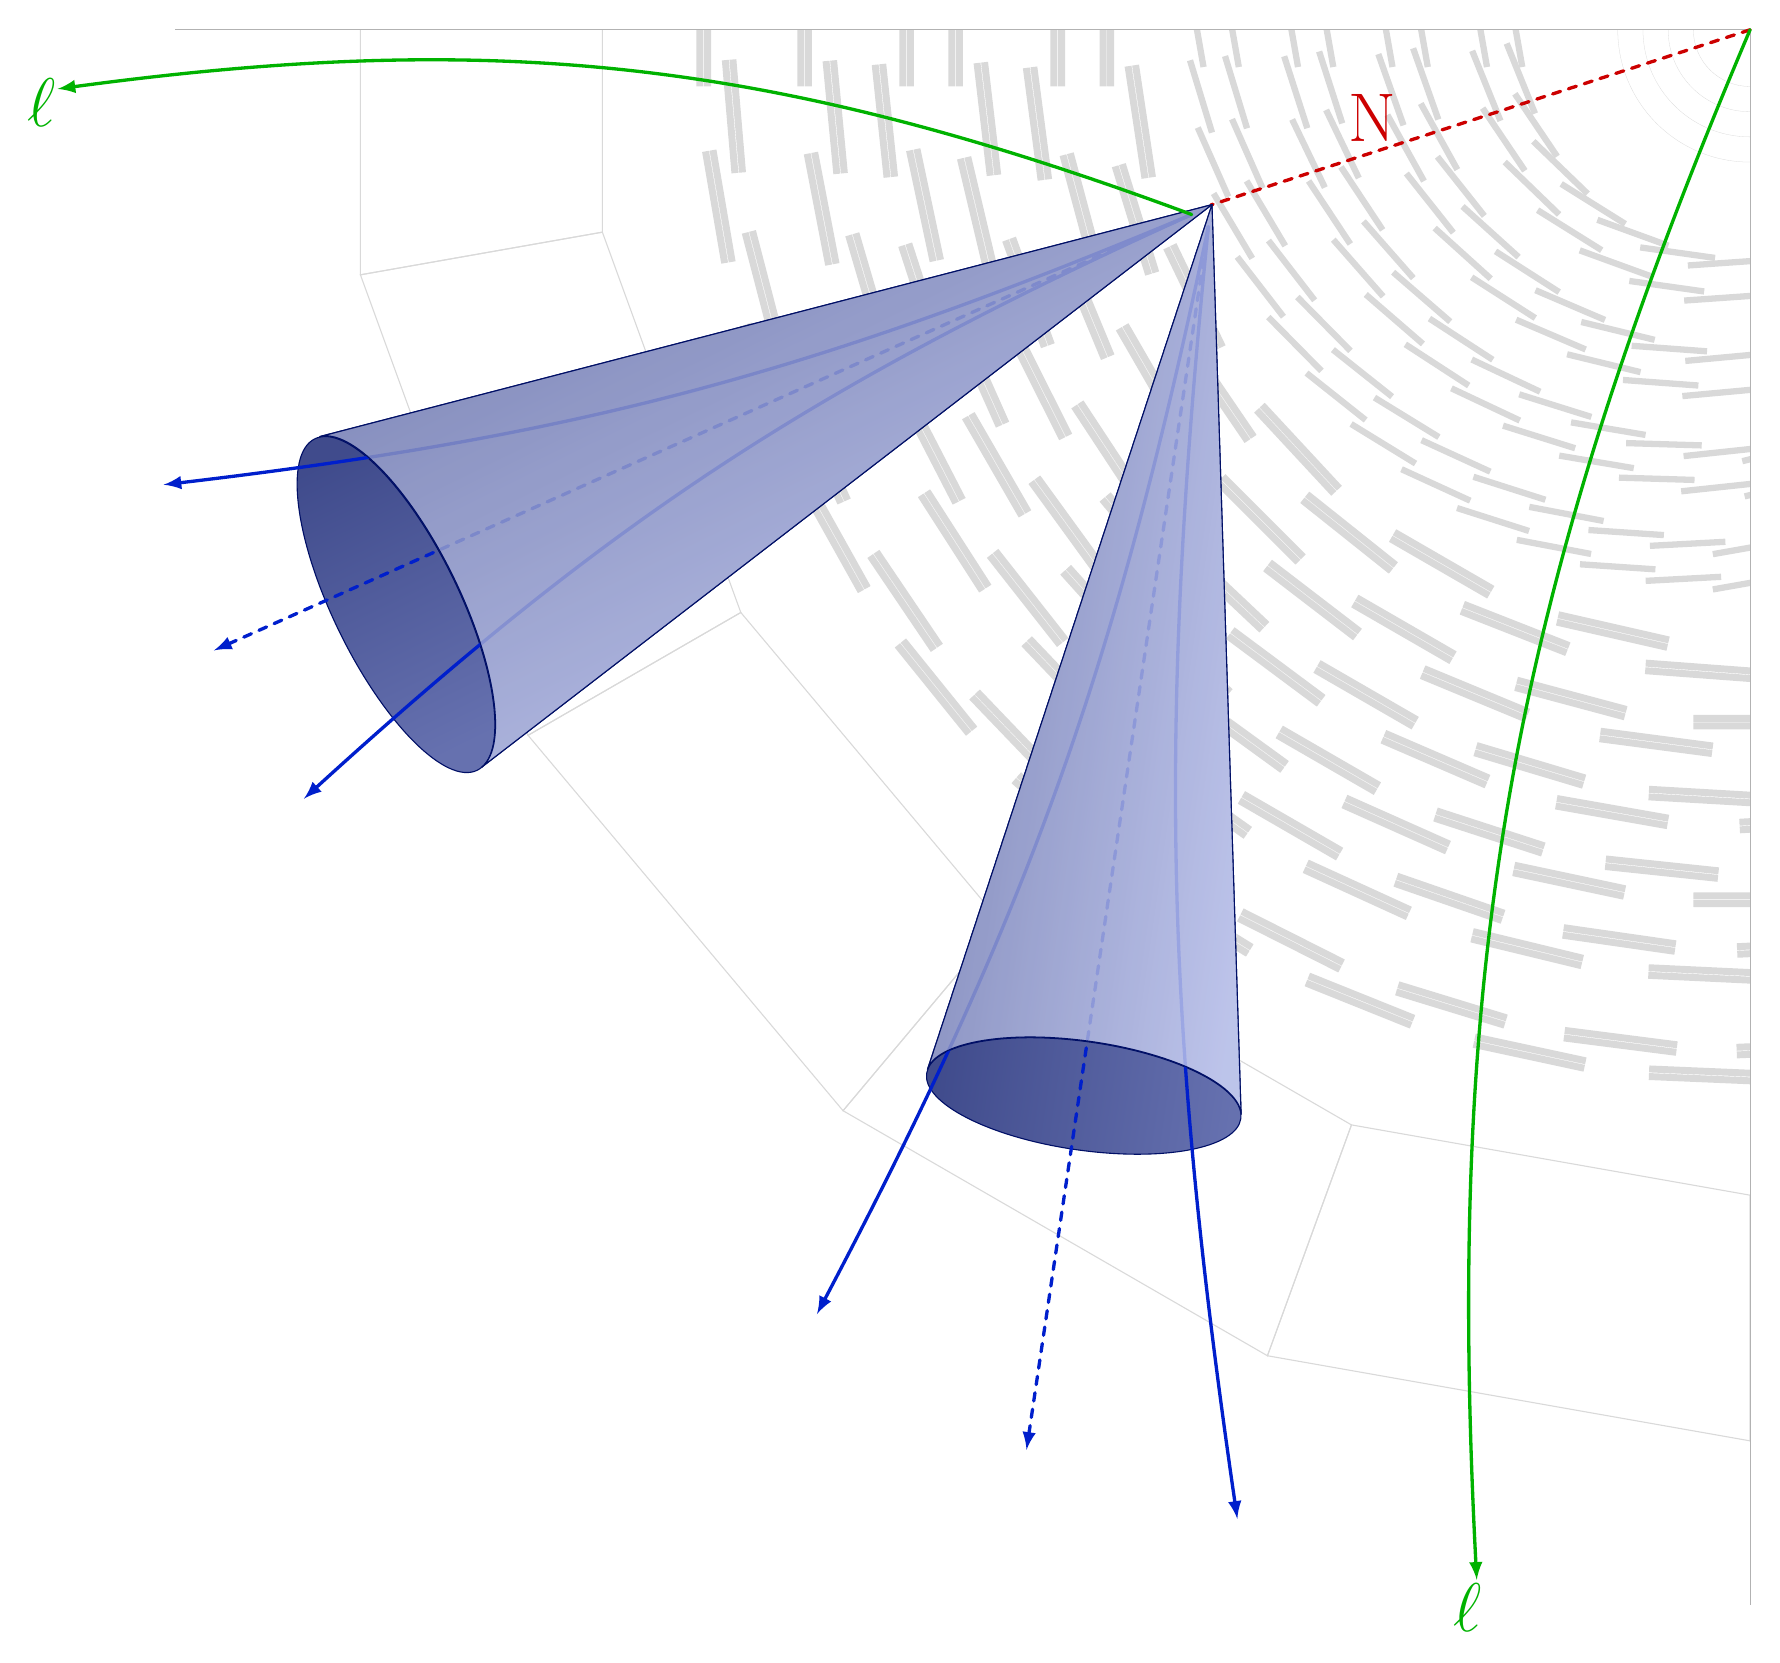
\begin{tikzpicture}[scale=5*\scale,
    rotate=0, 
    every node/.style={font=\fontsize{48}{14}\selectfont},
    % (you can still override per-path if needed)
]
  \def\angN{-162} % angle of HNL
  \def\lang{-100} % angle of HNL
  \def\dang{270} % angle of HNL
  \draw pic[black!15,scale=5*\scale] {detector={180:\dang}}; % \draw pic[black!15,scale=\scale] {detector={180:\dang}};
  \coordinate (PV) at (0,0); % primary vertex
  \draw[neutral exo, very thick] (PV) -- (\angN:0.90) coordinate (V)
    node[pos=0.7,above=0pt] {$\mathrm{N}$};
  \coordinate (J1) at (\angN+5:2.34); % displaced jet vector
  \coordinate (J2) at (\angN+40:2.00); % displaced jet vector
  \coordinate (L1) at (\lang:2.50);  % prompt lepton \coordinate (L1) at (\lang:2.50); 
  \coordinate (L2) at (\angN-16:2.69); % displaced lepton
  \draw[->,lepton, very thick] (PV) to[bend right=13] (L1) % prompt lepton
    node[anchor=172+\lang,inner sep=1pt] {$\ell$};

  \jetcone[quarkcol]{V}{J1}{23}{0.12}{ % displaced jet
    \draw[->,track, very thick] (V-v) to[bend right=9] (\angN+10:2.60);
    \draw[->,track,dashed, very thick] (V-v) -- (\angN+4:2.63);
    \draw[->,track, very thick] (V-v) to[bend left=8] (\angN-2:2.62);
  }

  \draw[->,lepton, very thick] (V-v) to[bend right=14] (L2) % displaced lepton
  node[anchor=40,inner sep=0pt] {$\ell$};

  \jetcone[quarkcol]{V}{J2}{20}{0.12}{ % displaced jet
    \draw[->,track, very thick] (V-v) to[bend left=8] (\angN+36:2.52);
    \draw[->,track,dashed, very thick] (V-v) -- (\angN+45:2.53);
    \draw[->,track, very thick] (V-v) to[bend right=7] (\angN+53:2.50);
  }
\end{tikzpicture}